\section{Simulation study}\label{sec:simulation}

We assess the procedure on synthetic scenes with known ground truth, where the
number of classes, the strength of spatial autocorrelation, the presence of a
trend, and the class separability are all controlled. The design isolates the
two failure modes of Section~\ref{subsec:null}, autocorrelation and
large-scale drift, and lets us verify the false-split control of
Proposition~\ref{prop:fpr} directly, by counting how often each method
recovers a single class when the scene contains exactly one.

\subsection{Generative model}\label{subsec:design}

All scenes live on a $96\times96$ lattice with $p=6$ bands. The elementary
building block is a unit-variance Gaussian random field
$g_\sigma$, obtained by convolving Gaussian white noise with an isotropic
Gaussian kernel of bandwidth $\sigma$ (which sets the autocorrelation range)
and standardising. Four world types instantiate the decomposition
\eqref{eq:decomp}:
\begin{description}
  \item[Null] ($K=1$): each band an independent $g_\sigma$,
        $\sigma\in\{3,6,9\}$. Pure autocorrelation, no discrete structure.
  \item[Trend] ($K=1$): each band $\theta\,t(s)+0.4\,g_3(s)$, with $t$ a
        standardised planar--bilinear polynomial surface and trend amplitude
        $\theta\in\{1.5,3.0\}$. Smooth large-scale variation, no classes.
  \item[Structured] ($K\in\{2,3,4,5\}$): a contiguous label map is drawn as
        the pixelwise $\argmax$ of $K$ independent fields $g_{\sigma_f}$,
        $\sigma_f\in\{6,9\}$; class $k$ is assigned a mean spectrum
        $\bm\mu_k\sim\mathcal N(\bm 0,\delta^2 I_p)$ with separation
        $\delta\in\{2,3,4\}$, and a per-band autocorrelated noise $g_2$ is
        added. Discrete classes embedded in autocorrelated noise.
  \item[Mixed] ($K\in\{3,4\}$): a structured scene ($\delta=3$, $\sigma_f=6$)
        plus a global polynomial trend of amplitude $\theta\in\{1.5,3.0\}$.
        The realistic case: classes \emph{and} drift together.
\end{description}
The factorial of these settings yields $33$ cells ($3$ null, $2$ trend, $24$
structured, $4$ mixed); each cell is realised $15$ times with independent
seeds, for $495$ scenes in total.

\subsection{Methods and metrics}\label{subsec:methods}

We compare fifteen criteria. Four are standard internal indices evaluated
against an independence null over $K=1,\dots,8$: the gap statistic
\citep{Tibshirani2001} with its Tibshirani rule, the average silhouette,
Calinski--Harabasz, and Davies--Bouldin. (The latter three cannot return
$K=1$ by construction, an asymmetry we return to below.) Two are the
calibrated-validity-index method of \citet{HennigLin2015}, the procedure
ESS-Dip extends: the average silhouette width calibrated by parametric
bootstrap against a null model, run both with an \emph{i.i.d.} Gaussian null
(the autocorrelation-blind application) and with a \emph{spatial} null
(phase-randomized surrogates preserving each band's variogram, their
autocorrelation-aware variant adapted to the gridded setting); $K$ is taken
where the calibrated index, in standard-deviation units, first exceeds a
significance threshold. A seventh baseline, plain \emph{dip-means}, applies the
same modality test at the nominal sample size, without the effective-sample-size
calibration, the local range, or the trend removal, isolating the contribution
of that spatial machinery. The eighth is the proposed method of
Section~\ref{sec:method}, denoted \textbf{ESS-Dip}:
Algorithm~\ref{alg:essdip} with the local within-class range
\eqref{eq:areamed}, adaptive trend removal \eqref{eq:detrendrule}, and a
$B=5$ ensemble; we fix $\alpha=0.05$, $\tau=0.25$, tile side $t=24$, and
$\nu=12$ throughout, with no per-scene tuning. The ninth, \textbf{ESS-Dip-R}, is
its recall-oriented variant: it calibrates the dip against the Gaussian null of
Assumption~\ref{ass:null} rather than the uniform least-favourable null, which is
less conservative and recovers more structure at the same specificity
(Section~\ref{subsec:simresults}). The remaining four are
ablations of ESS-Dip that disable one component each, to attribute the
contribution of every ingredient:
\emph{global range} (the $\ell^2$ range estimated over the whole image rather
than as a tile median); \emph{no trend removal}
($\tau=\infty$); \emph{forced trend removal} ($\tau=0$); and
\emph{declustering}, the precursor that subsamples the scene to one pixel per
decorrelation patch and applies the dip test to the thinned, approximately
independent sample. The fourteenth, \emph{SGS-Dip}, replaces the per-node
effective-sample-size calibration by the recursive Gaussian-simulation
reference \eqref{eq:sgstest} of Section~\ref{subsec:sgs} ($B=40$ simulations
per node); the fifteenth adds a Bonferroni multiple-testing correction to it.

Three metrics summarise performance. \emph{Specificity} is the fraction of
null and trend scenes (the $75$ scenes with $K=1$) for which $\hat K=1$; it is
the empirical analogue of Proposition~\ref{prop:fpr}. \emph{Exact-$K$ accuracy}
is the fraction of scenes with $\hat K=K_{\text{true}}$, reported separately
for the structured and mixed worlds, with the mean absolute error
$\mathrm{MAE}=\E\,\lvert\hat K-K_{\text{true}}\rvert$. The \emph{balanced
score} is the mean of specificity, structured accuracy and mixed accuracy, a
single figure that rewards methods strong across all three regimes rather than
in one.

\subsection{Results}\label{subsec:simresults}

Table~\ref{tab:bench} reports the three metrics; Figure~\ref{fig:bench}
displays the specificity--accuracy trade-off and the decay of accuracy with
the true number of classes.

\begin{table}[t]
\centering
\caption{Performance over the $495$ synthetic scenes. Specificity is the
$\hat K{=}1$ rate on the $75$ class-free (null${+}$trend) scenes; accuracy is
the exact-$K$ rate. Best in each column in bold.}
\label{tab:bench}
\begin{tabular}{l c cc c c}
\toprule
 & Specificity & \multicolumn{2}{c}{Structured} & Mixed & Balanced\\
\cmidrule(lr){3-4}
Method & ($\hat K{=}1$) & Acc. & MAE & Acc. & score\\
\midrule
\multicolumn{6}{l}{\textit{Standard internal indices (independence null)}}\\
Gap statistic            & 0.00 & \textbf{0.97} & \textbf{0.03} & 0.03 & 0.336\\
Silhouette               & 0.00 & 0.76 & 0.32 & 0.30 & 0.355\\
Calinski--Harabasz       & 0.00 & 0.85 & 0.18 & 0.40 & 0.418\\
Davies--Bouldin          & 0.00 & 0.70 & 0.41 & 0.20 & 0.299\\
\midrule
\multicolumn{6}{l}{\textit{Calibrated validity index} \citep{HennigLin2015}}\\
\quad i.i.d.\ null       & 0.00 & 0.67 & 0.42 & 0.17 & 0.280\\
\quad spatial null       & 0.80 & 0.72 & 0.38 & 0.17 & 0.561\\
\midrule
\multicolumn{6}{l}{\textit{Modality test without spatial calibration}}\\
Dip-means (nominal)      & 0.52 & 0.92 & 0.09 & 0.02 & 0.486\\
\midrule
\multicolumn{6}{l}{\textit{Proposed}}\\
ESS-Dip                  & \textbf{1.00} & 0.81 & 0.35 & 0.50 & 0.771\\
ESS-Dip-R (recall)       & \textbf{1.00} & 0.89 & 0.19 & \textbf{0.72} & \textbf{0.868}\\
\midrule
\multicolumn{6}{l}{\textit{Ablations of ESS-Dip}}\\
\quad global range       & 1.00 & 0.63 & 0.87 & 0.28 & 0.638\\
\quad no trend removal   & 1.00 & 0.63 & 0.89 & 0.13 & 0.587\\
\quad forced trend removal & 1.00 & 0.19 & 1.95 & 0.30 & 0.498\\
\quad declustering       & 1.00 & 0.63 & 0.83 & 0.08 & 0.572\\
\midrule
\multicolumn{6}{l}{\textit{Exact reference as a recursive estimator}}\\
SGS-Dip                  & 0.85 & 0.49 & 0.91 & 0.27 & 0.535\\
\quad + multiple-testing correction & 0.99 & 0.79 & 0.26 & 0.35 & 0.710\\
\bottomrule
\end{tabular}
\end{table}

\begin{figure}[t]
\centering
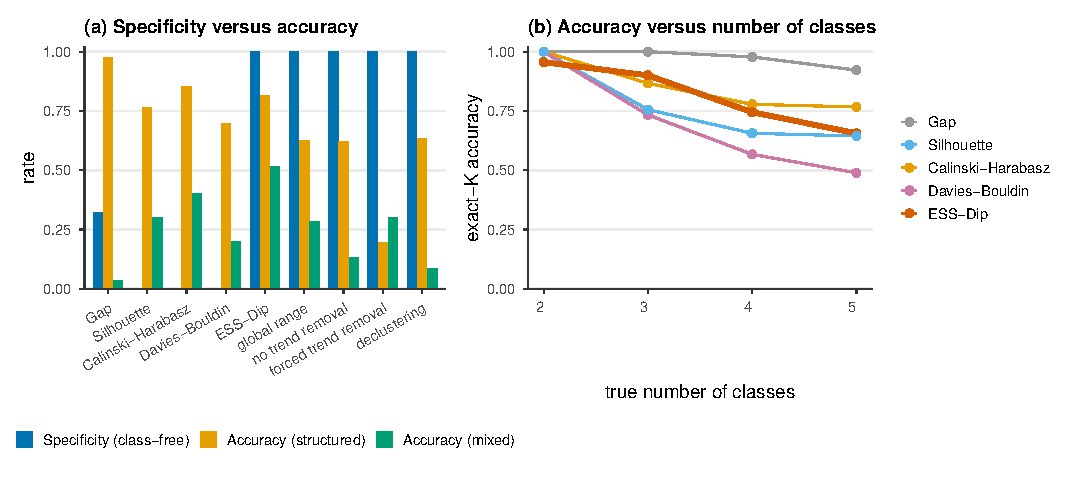
\includegraphics[width=\linewidth]{figures/benchmark.pdf}
\caption{Left: specificity (class-free scenes) against exact-$K$ accuracy on
structured and mixed scenes, by method. Only the proposed family attains unit
specificity; among them ESS-Dip recovers the most structure. Right: exact-$K$
accuracy versus the true number of classes on structured scenes. For legibility
the panels show the four standard indices and the ESS-Dip family; the
calibrated-validity-index and Gaussian-simulation methods of
Table~\ref{tab:bench} are omitted.}
\label{fig:bench}
\end{figure}

\paragraph{Standard indices over-detect without exception.}
On the $75$ class-free scenes every standard index reports spurious structure:
the $\hat K{=}1$ rate is $0.00$ for all four. The failure is severe, not
marginal: the gap statistic returns on average $\hat K=7.7$ classes on
fields that contain none, and the silhouette, Calinski--Harabasz and
Davies--Bouldin indices average $2.9$, $3.6$ and $4.1$. This is the
over-detection anticipated in Section~\ref{subsec:null}, now quantified: under
spatial autocorrelation an independence null cannot recognise the absence of
clusters.

\paragraph{The proposed family controls the false-split rate.}
Every member of the proposed family, ESS-Dip and all four ablations,
attains specificity $1.00$: in $75$ out of $75$ class-free scenes it returns a
single class. This is the empirical content of Proposition~\ref{prop:fpr}, and
it holds whether the class-free scene is stationary (null) or carries a smooth
drift (trend), confirming that the effective-sample-size calibration and the
adaptive detrending together neutralise both failure modes.

\paragraph{Specificity does not cost competitiveness.}
On the structured scenes the gap statistic is most accurate
($0.97$): with well-separated classes and an aligned null it is hard to beat,
and we do not. ESS-Dip reaches $0.81$, ahead of the silhouette ($0.76$),
Davies--Bouldin ($0.70$) and close to Calinski--Harabasz ($0.85$), while being
the \emph{only} method with non-zero specificity. On the realistic mixed
scenes ESS-Dip reaches $0.50$, ahead of every standard index ($0.40$ for the
best), because the adaptive detrending removes the drift that collapses them.
The recall variant ESS-Dip-R does better still: calibrating against the Gaussian
null of Assumption~\ref{ass:null} rather than the conservative uniform one, it
raises structured accuracy to $0.89$ and mixed accuracy to $0.72$ at the same
unit specificity, for a balanced score of $0.868$, the best of any method.
ESS-Dip itself scores $0.771$, already far above the next non-proposed method
($0.638$) and more than twice the best standard index ($0.418$). These synthetic
fields are Gaussian, so the model-matched ESS-Dip-R is favoured here; its
specificity and recall gains carry to the real scenes of
Section~\ref{sec:application}. Standard indices that look strong on pure
structured scenes collapse once specificity is taken into account.

\paragraph{Comparison with the method ESS-Dip extends.}
The calibrated-validity-index framework of \citet{HennigLin2015} is
instructive precisely because the present method generalises it. Applied with
an independence (i.i.d.) null it inherits the over-detection of the standard
indices (specificity $0.00$, balanced score $0.280$), confirming that the
framework alone, without a spatial null, does not address the problem. With its
autocorrelation-aware (spatial) null it recovers much of the lost specificity
($0.80$) and a comparable structured accuracy ($0.72$), a clear vindication of
its central idea. Two differences remain, and they are the contribution of this
paper. First, its specificity, at $0.80$, still admits one class-free scene in
five as clustered, where the within-class calibration of ESS-Dip admits none.
Second, and decisively, on the mixed regime its accuracy is only $0.17$,
no better than the i.i.d.\ variant and far below ESS-Dip's $0.50$, because a
phase-randomized null preserves the trend along with the autocorrelation and so
cannot separate a smooth drift from discrete classes. The explicit
trend--residual decomposition of Section~\ref{subsec:detrend}, absent from the
calibrated-index framework, is what closes this gap. This comparison is
insensitive to the significance threshold: the value used, $V>1.96$ (the
one-sided $2.5\%$ level for the calibrated index under approximate normality),
and the alternatives $V>1.64$ and $V>2.33$ all leave the conclusion intact:
the i.i.d.\ null fails specificity ($0.00$) at every threshold, and the spatial
null controls specificity ($0.77$--$0.83$) but not the mixed regime
($\le0.08$) at every threshold. Figure~\ref{fig:recover} makes the mixed-scene
behaviour concrete on one realisation: the gap statistic and the Hennig--Lin
null fragment the scene into six and eight clusters, whereas ESS-Dip recovers
the three true classes.

\begin{figure}[t]
\centering
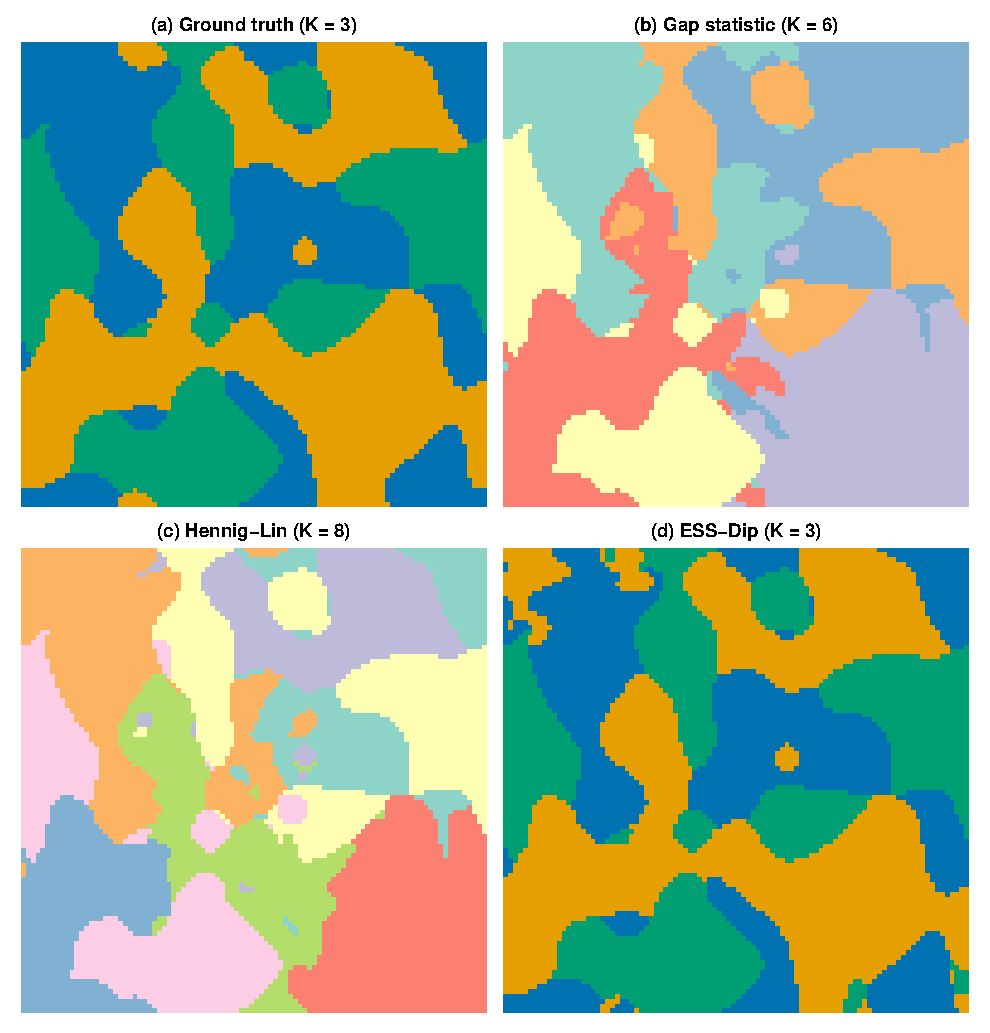
\includegraphics[width=\linewidth]{figures/recover.pdf}
\caption{Recovery on a representative mixed scene (three classes plus a smooth
trend). The gap statistic over-segments into six clusters (b) and the
Hennig--Lin spatial null into eight (c), both reading the trend and the
within-class autocorrelation as extra structure; ESS-Dip removes the trend and
calibrates to the effective sample size, recovering the three true classes (d),
whose partition matches the ground truth (a). Cluster colours in (b) and (c)
are arbitrary; in (a) and (d) they are matched, so a correct recovery
reproduces the colours of panel (a).}
\label{fig:recover}
\end{figure}

\subsection{Ablation}\label{subsec:ablation}

The ablations isolate where ESS-Dip's accuracy comes from
(Table~\ref{tab:bench}, lower block). The single largest contribution is the
\emph{local within-class range} of Section~\ref{subsec:range}: replacing it by
a scene-wide range drops structured accuracy from $0.81$ to $0.63$ and mixed
accuracy from $0.50$ to $0.28$. This confirms the diagnosis of
Section~\ref{subsec:range} (a global range conflates the between-class
mosaic with the within-class scale, inflating $\ell$, collapsing $\neff$, and
starving the test of power) while leaving specificity untouched.
\emph{Adaptive} trend removal matters in both directions: forcing detrending on
every scene ($\tau=0$) destroys structured accuracy ($0.19$), because the
polynomial absorbs genuine between-class signal when no trend is present;
disabling it ($\tau=\infty$) halves mixed accuracy ($0.13$), because an
unremoved drift inflates the range. Removing the drift \emph{only when present}
attains both ($0.81$ structured, $0.50$ mixed). The declustering precursor,
which discards all but one pixel per patch, matches the others on specificity
but trails on accuracy ($0.08$ mixed), confirming the value of calibrating on
the full pixel set rather than thinning it. At the opposite extreme, plain
dip-means (Table~\ref{tab:bench}) removes the spatial apparatus entirely and
applies the dip at the nominal size: the modality signal alone recovers
structure well ($0.92$, second only to the gap statistic), but without the
effective-sample-size calibration its specificity falls to $0.52$, and without
trend removal its mixed accuracy collapses to $0.02$. The contribution of
ESS-Dip is therefore not the modality test, which is already strong, but the
spatial calibration and trend separation that turn it from a high-recall,
low-specificity splitter into a precision-controlled homogeneity test, at a
modest cost in structured recall ($0.92$ to $0.81$).

\subsection{Geostatistical reference and the effective-sample-size
approximation}\label{subsec:geostat-ref}

Section~\ref{subsec:range} offers, alongside the default $1/e$-range proxy, a
fitted variogram and its integral range, and Section~\ref{subsec:sgs} offers the
exact
Gaussian-simulation reference \eqref{eq:sgstest} in place of the
effective-sample-size shortcut \eqref{eq:test}. Table~\ref{tab:geostat}
compares the three on one realisation of each world (six seeds, medians).

\begin{table}[t]
\centering
\caption{The decorrelation-area constant and the exact null. $\hat K$ under the
$\ell^2$ proxy and under the variogram integral range; and the
Gaussian-simulation homogeneity test \eqref{eq:sgstest} ($p$-value of the
leading split, $B=120$).}
\label{tab:geostat}
\begin{tabular}{l c cc c}
\toprule
 & & \multicolumn{2}{c}{$\hat K$} & SGS null \eqref{eq:sgstest}\\
\cmidrule(lr){3-4}
World & true $K$ & $a=\ell^2$ & integral range & $p$ (decision)\\
\midrule
Null    & 1 & 1 & 1 & 0.35\ \ ($K{=}1$)\\
Trend   & 1 & 1 & 1 & 0.46\ \ ($K{=}1$)\\
Struct  & 4 & 4 & 2 & 0.00\ \ ($K{\ge}2$)\\
Mixed   & 3 & 3 & 1 & 0.00\ \ ($K{\ge}2$)\\
\bottomrule
\end{tabular}
\end{table}

As a single homogeneity test the Gaussian-simulation reference
\eqref{eq:sgstest} is exactly right: it accepts homogeneity on the class-free
worlds ($p=0.35,0.46$) and rejects it on the structured and mixed worlds
($p<10^{-3}$), with no effective-sample-size approximation. The constant
$\kappa$ also matters: the mean-based integral range \eqref{eq:intrange} is some
three times larger than $\ell^2$ on these fields, so it is markedly more
conservative, preserving specificity but losing recall (structured $\hat K=2$,
mixed $\hat K=1$); the $\ell^2$ proxy is, for the dip, the better-calibrated of
the two scalar choices, consistent with the caveat of
Section~\ref{subsec:sgs} that an integral range derived for the sample mean
over-corrects a statistic of the empirical distribution, whose appropriate scale
is the smaller indicator integral range.

It is tempting to promote the exact reference to the estimator by calibrating
\emph{every} node of the recursion against simulations on its support. A direct
implementation (SGS-Dip, $B=40$) over-splits: specificity $0.85$, structured
accuracy $0.49$, balanced score $0.535$ against ESS-Dip's $0.771$
(Table~\ref{tab:bench}). This has two causes. First, the per-node test is
repeated across the recursion without correction, so the per-node level no
longer controls the family-wise false-split rate. Second, away from the leading
split a node is a spatially scattered subset whose variogram must be fitted on a
masked, non-rectangular support, biasing the simulated null.

The first cause is standard and correctable. A Bonferroni per-node level
$\alpha/K_{\max}$, with the matching number of simulations, restores specificity
to $0.99$ and lifts the balanced score to $0.710$, close to ESS-Dip's
$0.771$, the residual shortfall concentrated in the mixed regime
($0.35$ versus $0.50$; SGS-Dip\,+\,correction, Table~\ref{tab:bench}). So the
simulation null is a viable recursive estimator once multiple testing is
controlled. The second cause is more stubborn: on real imagery, where supports
are irregular and non-stationary, even the corrected estimator trails ESS-Dip:
single-class-window specificity $0.82$ and $0.98$ against $0.99$ and $1.00$
(Section~\ref{subsec:realspec}), and over-detection of full scenes. The
conclusion is therefore measured rather than categorical: the recursive
simulation null becomes competitive on controlled fields once corrected, but its
plug-in variogram on irregular supports, together with its cost of $B$
simulations per node against the cached, near-linear effective-sample-size
calibration, leaves \eqref{eq:test} the better practical choice. We retain it as
the method and use \eqref{eq:sgstest} as an assumption-light check on the
leading split.

\subsection{Computational performance}\label{subsec:timing}

Figure~\ref{fig:timing} reports single-threaded wall-clock time on structured
scenes. Across image sizes from $\sim\!2{,}300$ to $\sim\!66{,}000$ pixels,
ESS-Dip scales with an empirical exponent
$\mathrm{d}\log t/\mathrm{d}\log N = 0.86$ (panel~a), near-linear, consistent
with Section~\ref{subsec:complexity}, and is a constant factor (about
$1.2$--$2\times$) faster than the gap statistic, which scales similarly but
carries the overhead of its reference replicates. Cost grows sub-linearly with
the band count $p$ (panel~b: $0.31$\,s at $p=3$ to $1.02$\,s at $p=40$, at
$N=128^2$). Peak memory at $256\times256\times6$ is $8.9$\,MB, about three times
the input cube, so the method is memory-light at scene scale. The exact
Gaussian-simulation homogeneity test \eqref{eq:sgstest} with $B=120$ costs
$0.10$--$0.34$\,s over the same sizes, comparable to a single ESS-Dip
evaluation, as it concerns one node; a fully recursive simulation null would
multiply this by the number of nodes, which is the cost the
effective-sample-size calibration is designed to avoid.

\begin{figure}[t]
\centering
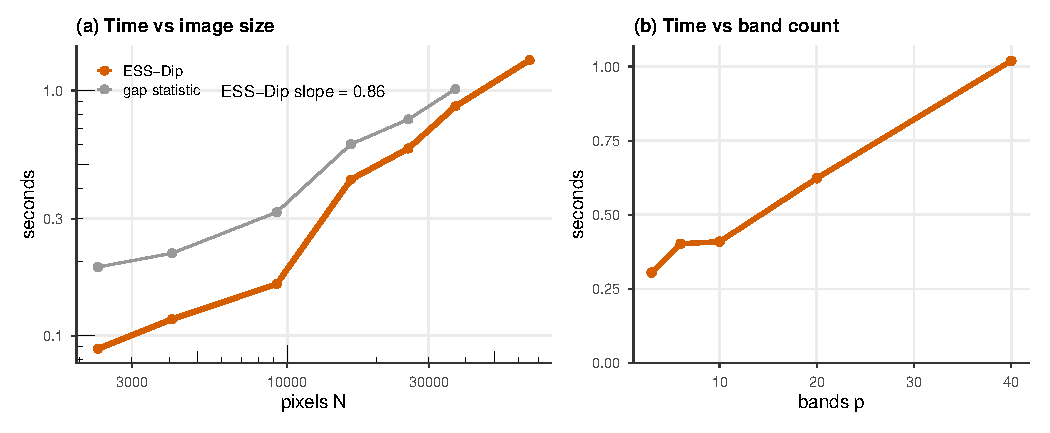
\includegraphics[width=\linewidth]{figures/timing.pdf}
\caption{Computational performance (single-threaded). (a) Wall-clock time
versus pixel count $N$ on a log--log scale, with the fitted ESS-Dip scaling
exponent; (b) time versus band count $p$ at $N=128^2$.}
\label{fig:timing}
\end{figure}

\subsection{Robustness to anisotropy}\label{subsec:aniso}

The decorrelation area \eqref{eq:areamed} is estimated from a radially averaged
(isotropic) variogram, yet directional autocorrelation does not degrade the
method. On null and structured worlds whose within-class range differs by a
factor of up to eight between the two axes, ESS-Dip retains specificity $1.00$
and structured accuracy $1.00$ at every anisotropy ratio tested ($1,2,4,8$),
whereas the gap statistic's specificity on the same class-free fields falls from
$0.88$ to $0.12$ as the field elongates. The isotropic scalar is thus an
adequate summary even under marked anisotropy, the modality signal it feeds
being direction-agnostic, and a fully anisotropic variogram
(Section~\ref{sec:discussion}) is a refinement rather than a necessity.
